
\part{Extending ImageJ\label{sec:Extending-ImageJ}}

ImageJ capabilities can be extended by loadable code modules in the
form of macros, scripts or plugins. 300$+$ macros, 500$+$ plugins
and 20$+$ scripts are available through the ImageJ web site. Below
is a short description of these three type of ImageJ add-ons:
\begin{lyxlist}{macrosss}
\item [{\nameref{sub:Macros-ExtendingIJ}}] \noindent The easiest way to
execute a series of ImageJ commands. The ImageJ \index{Macros}macro
language -- a \emph{Java-like} language -- contains a set of control
structures, operators and built-in functions and can be used to call
built-in commands and other macros. Macro code is stored in text files
(\filenameref{\noindent .txt} and \filenameref{\noindent .ijm} extensions).
\item [{\nameref{sub:Plugins}}] Much more powerful, flexible and faster
than macros (most of ImageJ's built-in menu commands are actually
\index{Plugins}plugins) but harder to write and debug. Plugins are
written in the \index{Java}Java programming language (\filenameref{.java}
source files) and compiled to \filenameref{.class} files.
\item [{\nameref{sub:Scripts}}] ImageJ uses the Mozilla Rhino interpreter
to run \index{JavaScript}JavaScripts. Similarly to plugins, scripts
have full access to all ImageJ and Java APIs but do not need to be
compiled (scripts and macros run interpretively). On the other hand,
scripts lack the simplicity of macro language and feel less integrated
in ImageJ.
\end{lyxlist}

\section{Macros\label{sub:Macros-ExtendingIJ}}

A \index{Macros}macro is a simple program that automates a series
of ImageJ commands. The easiest way to create a macro is to record
a sequence of commands using the command recorder (\textsf{\userinterface{\textsf{Plugins\lyxarrow{}Macros\lyxarrow{}}\nameref{sub:Record...}}}). 

A macro is saved as a text file (\filenameref{.txt }or \filenameref{.ijm}
extension) and once installed executed by selecting the macro name
in the \textsf{\userinterface{\textsf{Plugins\lyxarrow{}}\nameref{sub:Macros}}}
submenu, by \href{http://imagej.nih.gov/ij/developer/macro/macros.html\#shortcuts}{pressing a key}
or, in the case of \href{http://imagej.nih.gov/ij/developer/macro/macros.html\#tools}{Macro tools},
by clicking on an icon in the ImageJ toolbar. In addition, any macro
file placed in \dirnameref{ImageJ/plugins} with an \filenameref{.ijm}
extension will be installed in the \textsf{\userinterface{\textsf{Plugins\lyxarrow{}}}
}menu like any other plugin (before version\,1.41 only files with
an underscore in the name would be listed).

There are more than 300\,example macros, on the ImageJ Web site.
To try one, open it in a browser window and drag it directly to the
\nameref{fig:The-ImageJ-window} or, copy it to the clipboard (\mykeystroke{Ctrl}
\mykeystroke{A}, \mykeystroke{Ctrl} \mykeystroke{C}), switch to
IJ, and run \textsf{\userinterface{\textsf{File\lyxarrow{}New\lyxarrow{}}\nameref{sub:SystemClipboard[V]}}}
(\mykeystroke{Ctrl} \mykeystroke{Shift} \mykeystroke{V}), pasting
the macro into a new \nameref{sub:ImageJ-Macro-Editor} window. Run
it using the editor's \textsf{Macros\lyxarrow{}Run Macro} command
(\mykeystroke{Ctrl} \mykeystroke{R}). Most of the example macros
are also available in the macros folder, inside the ImageJ folder.


\subsection*{Macro Programming\label{sub:Macro-Programming}}

The ImageJ community has created excellent tutorials on macro programming.
These resources are indispensable guides to the ImageJ macro language: 
\begin{enumerate}
\item \emph{The ImageJ Macro Language --- Programmer's Reference Guide}
by J�r�me Mutterer and Wayne Rasband. This booklet compiles most of
the documentation dispersed throughout the web related to ImageJ's
macro programming. It provides an up to date printable manual for
the ImageJ macro language:\\
\url{http://imagej.nih.gov/ij/docs/macro_reference_guide.pdf}
\item \improvement{Fourtneen new macro functions}The Built-in Macro Functions
webpage (\textsf{\userinterface{\textsf{Help\lyxarrow{}}\nameref{sub:Macro-Functions...}}}
and \textsf{\userinterface{\textsf{Macros\lyxarrow{}}\nameref{FunctionFinder[F]}}}
in the \nameref{sub:ImageJ-Macro-Editor}), the indispensable guide
to the built-in functions that can be called from the ImageJ macro
language. It is thoroughly documented and constantly updated:\\
\url{http://imagej.nih.gov/ij/developer/macro/functions.html}
\item Tutorials on the \index{Fiji}Fiji webpage: \\
\url{http://fiji.sc/wiki/index.php/Introduction_into_Macro_Programming}
\item How-tos and tutorials on the ImageJ Documentation Portal\\
\url{http://imagejdocu.tudor.lu/}
\end{enumerate}

\calso{\nameref{sub:Scripts}, \nameref{sub:Plugins}, \nameref{sub:ImageJ-Macro-Editor},
\nameref{sub:Fiji-Scrip-Editor}}


\section{Scripts\label{sub:Scripts}}

\index{JavaScript}JavaScript scripting was introduced in ImageJ\,1.41
in order to bring full access to ImageJ and Java APIs (\emph{see}
\nameref{tab:Advantages-JavaScript}). ImageJ uses the Mozilla Rhino
interpreter built into Java\,1.6 for Linux and Windows to run JavaScript.
Mac users, and users of earlier versions of Java, must download \filenameref{JavaScript.jar}
into the plugins folder. This JAR\nomenclature{JAR}{Java ARchive}
file is available on the \href{http://imagej.nih.gov/ij/download/tools/JavaScript.jar}{ImageJ website}
and is included with the Mac version of ImageJ in \dirnameref{ImageJ/plugins/jars}. 

Example JavaScript programs are available at \href{http://imagej.nih.gov/ij/macros/js/}{imagej.nih.gov/ij/macros/js/}.
Thread safe JavaScript code can be generated using the Recorder (\userinterface{Plugins\lyxarrow{}Macros\lyxarrow{}\nameref{sub:Record...}}).
Scripts can be opened in the editor as any other macro. Scripts with
the extension \filenameref{.js} can be run using \userinterface{Macros\lyxarrow{}Run Macro}
otherwise \userinterface{Macros\lyxarrow{}Evaluate JavaScript} (\mykeystroke{Ctrl}
\mykeystroke{J}) must be used.


\subsection*{JavaScript Programming}

Resources on ImageJ JavaScript scripting include:
\begin{enumerate}
\item The ImageJ web site, with growing documentation:\\
\url{http://imagej.nih.gov/ij/developer/javascript.html}
\item Tutorials on the \index{Fiji}Fiji webpage:\\
\url{http://fiji.sc/wiki/index.php/Javascript_Scripting}
\item Online scripts repository:\\
\url{http://imagej.nih.gov/ij/macros/js/}
\end{enumerate}
\selectlanguage{american}%
\begin{table}
\noindent \caption[\selectlanguage{english}%
Advantages and disadvantages of JavaScript\selectlanguage{english}%
]{\selectlanguage{english}%
\label{tab:Advantages-JavaScript}\textbf{Advantages and disadvantages
of JavaScript in ImageJ.} \index{ActionBar}\index{CodeBar} A thorough
comparison between different scripting languages is available on the
\protect\href{http://fiji.sc/wiki/index.php/Scripting_comparisons}{Fiji webpage}.\selectlanguage{english}%
}


\noindent {\scriptsize }%
\begin{minipage}[t]{1\columnwidth}%
\selectlanguage{english}%
\renewcommand{\arraystretch}{1.15}
\addtocounter{footnote}{1}
\begin{spacing}{0.9}

\noindent %
\begin{tabular}{>{\raggedright}p{0.476\columnwidth}>{\raggedright}p{0.476\columnwidth}}
\toprule 
\multicolumn{1}{>{\centering}m{0.476\columnwidth}}{{\small JavaScript Advantages}} & \multicolumn{1}{>{\centering}m{0.476\columnwidth}}{{\small JavaScript Disadvantages}}\tabularnewline
\midrule
{\small Full access to ImageJ and Java APIs} & {\small Slower, especially starting up}\tabularnewline
{\small \href{http://en.wikipedia.org/wiki/ECMAScript}{Standardized}} & {\small No equivalent of macro sets}\tabularnewline
{\small Richer language (objects, \code{{\small ?}} operator, \code{{\small break}},
\code{{\small continue}}, etc.)} & {\small Cannot use most of ImageJ's 360+ \href{http://imagej.nih.gov/ij/developer/macro/functions.html}{built in macro functions}}\tabularnewline
{\small \href{http://en.wikipedia.org/wiki/JavaScript}{Extensive documentation}} & {\small Requires knowledge of complex ImageJ and Java APIs}\tabularnewline
 & {\small No support for ``batch mode''}\tabularnewline
 & {\small Cannot create tools and toolbar menus}\tabularnewline
 & {\small Not compatible with Function Finder and CodeBar}%
\footnote{{\small CodeBar is a convenient `ActionBar' that retrieves snippets
and common tasks frequently used in macro writing. `ActionBars'
provide one or many easy to use button bar(s) that extend ImageJ's
graphical user interface. You can read more about the ActionBar plugin
at the \href{http://imagejdocu.tudor.lu/doku.php?id=plugin:utilities:action_bar:start}{ImageJ Documentation Portal}.}%
}\tabularnewline
 & {\small No debugger}\tabularnewline
\end{tabular}

\end{spacing}\selectlanguage{english}%
%
\end{minipage}
\end{table}


\selectlanguage{english}%

\calso{\nameref{sub:Macros-ExtendingIJ}, \nameref{sub:Plugins}, \nameref{sub:ImageJ-Macro-Editor},
\nameref{sub:Fiji-Scrip-Editor}}


\section{Plugins\label{sub:Plugins}}

Plugins are a much more powerful concept than \nameref{sub:Macros-ExtendingIJ}
and \nameref{sub:Scripts} and most of ImageJ's built-in menu commands
are in fact implemented as \index{Plugins}plugins. Quoting Werner
Bailer \cite{Bailer:2006p14110}:
\begin{quotation}
Plugins are implemented as \index{Java}Java classes, which means
that you can use all features of the Java language, access the full
ImageJ API\nomenclature{API}{Application Programming Interface} and
use all standard and third-party Java APIs in a plugin. This opens
a wide range of possibilities of what can be done in a plugin. 

The most common uses of plugins are filters performing some analysis
or processing on an image or image stack and I/O plugins for reading/writing
not natively supported formats from/to file or other devices. But
as you can see when looking at the plugins listed on the ImageJ plugins
page, there are many other things you can do with plugins, such as
rendering graphics or creating extensions of the ImageJ graphical
user interface.
\end{quotation}
Plugins in the \dirnameref{ImageJ/plugins/} folder are listed at
the bottom of the \userinterface{\nameref{sec:Plugins}} menu (\emph{see}
\ref{infobox:Organizing-Commands} \nameref{infobox:Organizing-Commands}).
Only \filenameref{.class} and \filenameref{.jar} files in the plugins
folder with at least one underscore in their name will be installed.
Note that, with IJ\,1.44d an later, ImageJ no longer automatically
installs, at startup, plugins in JAR file directories that start with
a lower case letter. 


\subsection*{Developing ImageJ Plugins}

More information on how to develop ImageJ plugins can be obtained
on the following documents:
\begin{enumerate}
\item Developer Resources Page on the ImageJ website (\textsf{\userinterface{\textsf{Help\lyxarrow{}}\nameref{sub:Help-Dev.Resources...}}}):\\
\url{http://imagej.nih.gov/ij/developer/index.html}
\item Dedicated tutorials on \index{Fiji}Fiji's webpage:\\
\url{http://fiji.sc/wiki/index.php/Introduction_into_Developing_Plugins}
\item Dedicated tutorials on the ImageJ Documentation Portal:\\
\url{http://imagejdocu.tudor.lu/}
\item Dedicated tutorials on the ImageJDev webpage:\nomenclature{IDE}{Integrated Development Environment}\index{Eclipse}\index{NetBeans}\\
\url{http://developer.imagej.net/ides}
\end{enumerate}

\calso{\nameref{sub:Macros-ExtendingIJ}, \nameref{sub:Scripts}, \nameref{sub:ImageJ-Macro-Editor},
\nameref{sub:Fiji-Scrip-Editor}}


\section{Scripting in Other Languages\label{sec:ScriptingOtherLang}}

Support for other languages is possible in ImageJ using \nameref{sub:Fiji-intro}
and its powerful editor. Fiji adds extra support for \index{BeanShell}BeanShell,
\index{Clojure}Clojure, \index{Python}\index{Jython@Jython  \see{Python,}}Python
and \index{Ruby}Ruby. The following documents will introduce you
to the advanced scripting capabilities of Fiji:
\begin{enumerate}
\item The extensive tutorial on scripting Fiji with Jython by Albert Cardona:\\
\url{http://www.ini.uzh.ch/~acardona/fiji-tutorial/}
\item Dedicated tutorials on the \index{Fiji}Fiji webpage:\\
\url{http://fiji.sc/wiki/index.php/Scripting_comparisons}
\end{enumerate}

\subsection*{Fiji Script Editor\label{sub:Fiji-Scrip-Editor}}

Fiji features a more powerful script editor than ImageJ's built-in
\nameref{sub:ImageJ-Macro-Editor}. The Fiji editor is an invaluable
help when writing scripts in any of Fiji's supported languages, including
the ImageJ macro language. The editor features full undo support,
\index{Syntax highlighting}syntax highlighting, tabs, bookmarks and
several other tools that simplify scripting workflows in ImageJ. For
more information visit Fiji's editor website at \url{http://fiji.sc/wiki/index.php/Script_Editor}.

\begin{figure}[h]
\noindent 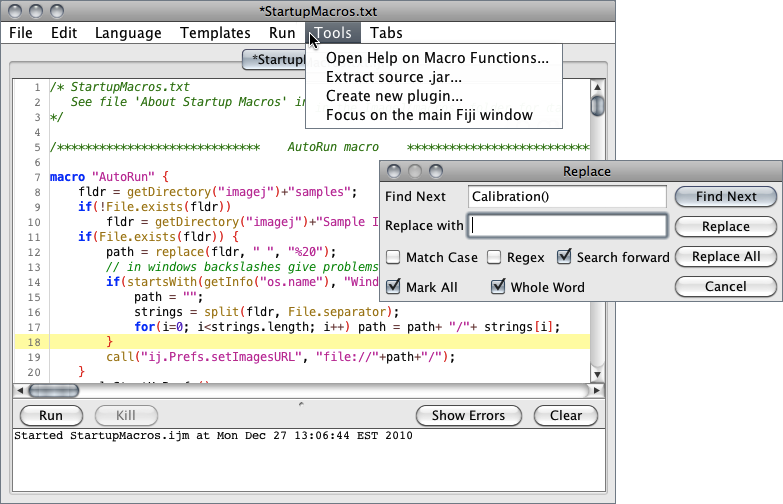
\includegraphics[scale=0.45]{images/FijiScriptEditor}\caption{\textbf{\label{fig:Fiji-Script-Editor}The Fiji Script Editor (ImageJA\ 1.44m).
}The Fiji Editor is an advanced text editor, supporting BeanShell,
Jython, JRuby and other scripting languages. It does not support \protect\userinterface{\nameref{FunctionFinder[F]}}
but selecting a built-in macro function and running \protect\userinterface{Tools\lyxarrow{}Open Help on Macro Functions\ldots{}}
retrieves the documentation for the selected function.}
\end{figure}



\calso{\noindent \nameref{sec:ScriptingOtherLang}, \nameref{sub:IJ-cmd-line},
\href{http://imagejdocu.tudor.lu/doku.php?id=plugin:utilities:ij_ed:start}{IJ\_{}ED},
a plugin by J�r�me Mutterer that binds \href{http://www.jedit.org/}{jEdit}
to ImageJ }


\section[Running ImageJ From the Command Line]{Running ImageJ from the Command Line\label{sub:IJ-cmd-line}}

ImageJ was devised as a desktop application. It can, however, run
without a graphics environment (\index{Headless mode}headless mode)
by adding a special library (\code{headless.jar}) to the \code{ij.jar}
classpath that overrides key ImageJ classes to work better headlessly.
As described on the \href{http://fiji.sc/wiki/index.php/Headless}{Fiji website},
this strategy is implemented in \nameref{sub:Fiji-intro} through
the \code{-}\code{-headless} command line flag (\emph{see also}
\href{http://imagejdocu.tudor.lu/doku.php?id=faq:technical:how_do_i_run_imagej_without_a_graphics_environment_headless}{Running ImageJ in headless mode}
and \href{http://cmci.embl.de/documents/100922imagej_cluster}{Using Cluster for Image Processing with IJ}).
Headless operations are simplified in \nameref{sub:ImageJ2intro}.

ImageJ recognizes the following command line options:

\begingroup
%change ttvariant to courier since default monospaced font does not allow bold typeface
\renewcommand{\ttdefault}{pcr}

\begin{lyxlist}{eval-macro-code-batch-pat}
\item [{\texttt{\textbf{\code{\noindent \texttt{\textbf{\textquotedbl{}file-name}}\texttt{\textquotedbl{}}}}}}] \noindent Opens
a file. Examples:\\
\texttt{\hspace*{15pt}\code{\noindent \texttt{blobs.tif}}}\\
\texttt{\hspace*{15pt}\code{\noindent \texttt{/Users/wayne/images/blobs.tif}}}\\
\texttt{\hspace*{15pt}\code{\noindent \texttt{e81{*}.tif}}}
\item [{\texttt{\textbf{-ijpath\ path}}}] \noindent Specifies the path
to the directory containing the plugins directory. Example:\\
\texttt{\hspace*{15pt}\code{\noindent \texttt{-ijpath /Applications/ImageJ}}}
\item [{\texttt{\textbf{-port}}}] \noindent Specifies the port ImageJ uses
to determine if another instance is running. Examples:\texttt{}~\\
\texttt{\hspace*{15pt}\code{\noindent \texttt{-port1}}} (use default
port address + 1) \\
\texttt{\hspace*{15pt}\code{\noindent \texttt{-port2}}} (use default
port address + 2)\\
\texttt{\hspace*{15pt}\code{\noindent \texttt{-port0}}} (do not
check for another instance (\href{http://imagej.nih.gov/ij/source/ij/OtherInstance.java}{OtherInstance})
\item [{\texttt{\textbf{-macro\ path\ {[}arg{]}}}}] \noindent Runs a
macro or script, passing it an optional argument, which can be retrieved
using \texttt{getArgument()}. Examples:\\
\texttt{\hspace*{15pt}\code{\noindent \texttt{-macro analyze.ijm}}}\\
\texttt{\hspace*{15pt}\code{\noindent \texttt{-macro analyze /Users/wayne/images/stack1} }}
\item [{\texttt{\textbf{-batch\ path\ {[}arg{]}}}}] \noindent Runs a
macro or script in batch mode (no GUI), passing it an optional argument.
ImageJ exits when the macro finishes.
\item [{\texttt{\textbf{-eval\ \textquotedbl{}macro\ code\textquotedbl{}}}}] \noindent Evaluates
macro code. Examples:\\
\texttt{\hspace*{15pt}\code{\noindent \texttt{-eval \textquotedbl{}print(\textquotesingle{}Hello,
world\textquotesingle{});\textquotedbl{}}}}\\
\texttt{\hspace*{15pt}\code{\noindent \texttt{-eval \textquotedbl{}return getVersion();\textquotedbl{}}}}
\item [{\texttt{\textbf{-run\ command}}}] \noindent Runs an ImageJ menu
command. Example:\\
\texttt{\hspace*{15pt}\code{\noindent \texttt{-run \textquotedbl{}About ImageJ\ldots{}\textquotedbl{}}}}
\item [{\texttt{\textbf{-debug}}}] \noindent Runs ImageJ in debug mode.
\end{lyxlist}
\endgroup


\calso{\href{http://imagej.nih.gov/ij/docs/install/linux.html}{Linux installation},
\href{http://imagejdocu.tudor.lu/doku.php?id=diverse:start&s[]=command&s[]=line}{ImageJ Documentation Portal: Command line}}
